% Demo paper for samepage's README and screenshots. Written for this repository (AGPL-3.0-only,
% like the project); the study and its data are fictional. Compile: tectonic demo-paper.tex
\documentclass[10pt,a4paper,twocolumn]{article}
\usepackage{fontspec}
\usepackage[turkish,shorthands=off]{babel}
\usepackage{amsmath}
\usepackage{booktabs}
\usepackage{tikz}
\usepackage{xcolor}
\usepackage[margin=1.8cm,columnsep=0.6cm]{geometry}
\usepackage{fancyhdr}
\usepackage[hidelinks]{hyperref}
\definecolor{accent}{HTML}{0B7A3E}
\pagestyle{fancy}
\fancyhf{}
\fancyhead[L]{\small Örnek Bilimler Dergisi, 1(1), 2026}
\fancyhead[R]{\small Yılmaz ve Demir}
\fancyfoot[C]{\small\thepage}
\renewcommand{\headrulewidth}{0.4pt}
\begin{document}
\twocolumn[{%
\begin{center}
{\LARGE\bfseries Akademik Metinlerin Makine Çevirisinde\\ Anlam Kaymasının Ölçülmesi\par}
\vspace{0.8em}
{\large Ayşe Yılmaz\textsuperscript{1}, Mehmet Demir\textsuperscript{2}\par}
\vspace{0.4em}
{\small \textsuperscript{1}Örnek Üniversitesi, Bilgisayar Mühendisliği Bölümü; ayse.yilmaz@example.org\\
\textsuperscript{2}Örnek Teknik Üniversitesi, Mütercim ve Tercümanlık Bölümü; mehmet.demir@example.org\par}
\end{center}
\vspace{0.6em}
\noindent\colorbox{accent!8}{\parbox{\dimexpr\textwidth-2\fboxsep}{%
\vspace{0.3em}\textbf{Öz.} Makine çevirisi akademik yayıncılıkta giderek daha sık kullanılmaktadır;
ancak çevirinin metnin anlamını koruyup korumadığı çoğu zaman denetlenmemektedir. Bu çalışmada
2019–2023 yılları arasında yayımlanmış 412 Türkçe makalenin özetleri İngilizceye çevrilmiş ve
18.640 tümce iki bağımsız uzman tarafından anlam kayması açısından incelenmiştir. Uzmanlar
arasındaki uyum katsayısı $\kappa = 0{,}81$ olarak hesaplanmıştır. Bulgular, olumsuzluk ve
kesinlik bildiren ifadelerin çeviride en sık kaybolan öğeler olduğunu göstermektedir. Terim
tutarlılığı kısa tümcelerde \%92,1 iken kırk sözcükten uzun tümcelerde \%71,2'ye düşmüştür
($p < 0{,}01$). Sonuçlar, geri çeviriyle yapılan otomatik bir denetimin anlam kaymalarının büyük
bölümünü yakalayabileceğine işaret etmektedir.\\[0.4em]
\textbf{Anahtar Kelimeler:} makine çevirisi, anlam kayması, akademik yazım, geri çeviri, terim
tutarlılığı\vspace{0.3em}}}
\vspace{1.2em}
}]
\renewcommand{\thefootnote}{}
\footnotetext{Bu belge samepage'in tanıtımı için hazırlanmış kurgusal bir örnektir; çalışma ve
verileri gerçek değildir.}
\renewcommand{\thefootnote}{\arabic{footnote}}

\section{Giriş}
Sinir ağı tabanlı makine çevirisi sistemleri, tümce düzeyindeki bağlamı dikkate aldıkları için
önceki yöntemlere göre çok daha akıcı çeviriler üretmektedir [1, 2]. Ne var ki akıcılık
doğruluğun güvencesi değildir: akademik bir metinde tek bir olumsuzluk ekinin ya da kesinlik
derecesini bildiren bir ifadenin kaybolması, bulgunun anlamını tümüyle değiştirebilir. Örneğin
\textit{sonuçlar bir etkinin olabileceğini düşündürmektedir} tümcesi \textit{sonuçlar etkiyi
kanıtlamaktadır} biçiminde çevrildiğinde yazarın temkinli tutumu ortadan kalkar.

Bu çalışmanın amacı, Türkçe akademik metinlerin İngilizceye çevirisinde ortaya çıkan anlam
kaymalarını sınıflandırmak ve bu kaymaların ne ölçüde otomatik olarak saptanabileceğini
göstermektir.\footnote{Derlemdeki tümceler yalnızca araştırma amacıyla kullanılmıştır.}

\section{Yöntem}
Derlem, açık erişimli Türkçe dergilerden seçilen 412 makalenin özet, giriş ve sonuç
bölümlerinden oluşmaktadır. Her tümce iki uzman tarafından dört kategoriden birine atanmıştır:
anlam korunmuş, olumsuzluk kaybı, kesinlik kaybı ve terim hatası. Uzmanlar arasındaki uyum
Cohen'in kappa katsayısıyla ölçülmüştür [3].

Otomatik denetimin başarımı, kesinlik $P$ ve duyarlılık $R$ değerlerinin harmonik ortalaması olan
\begin{equation}
F_1 = \frac{2PR}{P+R}
\end{equation}
ölçütüyle hesaplanmıştır. Çeviri kalitesi ayrıca BLEU puanıyla raporlanmıştır [4].

\section{Bulgular}
Tablo~1'de görüldüğü üzere tümcelerin \%87,4'ünde anlam korunmuştur. Anlam kaymalarının en sık
görülen türü olumsuzluk kaybıdır; bunu kesinlik kaybı izlemektedir.

\begin{table}[h]
\centering
\caption{Anlam kayması türlerinin dağılımı.}
\begin{tabular}{lrr}
\toprule
Kategori & Tümce & Oran (\%) \\
\midrule
Anlam korunmuş & 16.290 & 87,4 \\
Olumsuzluk kaybı & 1.118 & 6,0 \\
Kesinlik kaybı & 857 & 4,6 \\
Terim hatası & 375 & 2,0 \\
\midrule
Toplam & 18.640 & 100,0 \\
\bottomrule
\end{tabular}
\end{table}

Şekil~1, terim tutarlılığının tümce uzunluğu arttıkça belirgin biçimde azaldığını
göstermektedir. Kısa ve uzun tümceler arasındaki fark istatistiksel olarak anlamlıdır
($p < 0{,}01$).

\begin{figure}[h]
\centering
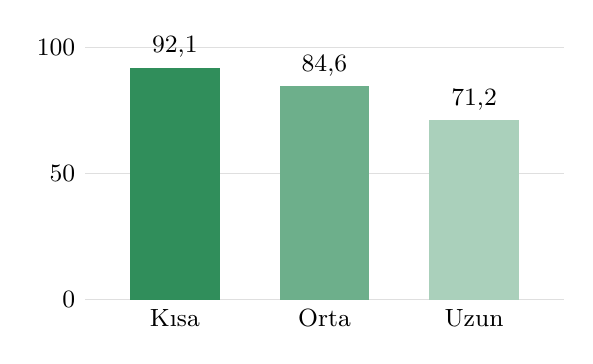
\begin{tikzpicture}[x=1.9cm,y=0.032cm]
\draw[gray!60] (0.4,0) -- (3.6,0);
\foreach \v in {0,50,100} {\draw[gray!25] (0.4,\v) -- (3.6,\v); \node[left,font=\small] at (0.4,\v) {\v};}
\fill[accent!85] (0.7,0) rectangle (1.3,92.1);
\fill[accent!60] (1.7,0) rectangle (2.3,84.6);
\fill[accent!35] (2.7,0) rectangle (3.3,71.2);
\node[above,font=\small] at (1,92.1) {92,1};
\node[above,font=\small] at (2,84.6) {84,6};
\node[above,font=\small] at (3,71.2) {71,2};
\node[below,font=\small] at (1,0) {Kısa};
\node[below,font=\small] at (2,0) {Orta};
\node[below,font=\small] at (3,0) {Uzun};
\end{tikzpicture}
\caption{Tümce uzunluğuna göre terim tutarlılığı (\%).}
\end{figure}

\section{Tartışma}
Geri çeviriyle yapılan denetim, olumsuzluk kayıplarının \%91'ini ve kesinlik kayıplarının
\%78'ini doğru biçimde işaretlemiştir. Kesinlik bildiren ifadeler dilden dile farklı biçimlerde
kurulduğundan bu türdeki kayıpların saptanması daha güçtür. Yine de bulgular, yazar tarafından
yapılacak hedefli bir gözden geçirmenin anlam kaymalarının büyük bölümünü giderebileceğini
düşündürmektedir.

\section{Sonuç}
Bu çalışma, akademik metinlerin makine çevirisinde anlam kaymalarının azımsanmayacak sıklıkta
görüldüğünü ve bunların önemli bir bölümünün otomatik olarak saptanabildiğini göstermektedir.
Gelecek çalışmalarda derlemin başka dil çiftlerine genişletilmesi planlanmaktadır.

\section*{Kaynaklar}
{\small
\noindent[1] Vaswani, A., Shazeer, N., Parmar, N., Uszkoreit, J., Jones, L., Gomez, A. N.,
Kaiser, Ł. ve Polosukhin, I. (2017). Attention is all you need. \textit{Advances in Neural
Information Processing Systems}, 30.

\noindent[2] Koehn, P. (2010). \textit{Statistical Machine Translation}. Cambridge University
Press.

\noindent[3] Cohen, J. (1960). A coefficient of agreement for nominal scales. \textit{Educational
and Psychological Measurement}, 20(1), 37–46.

\noindent[4] Papineni, K., Roukos, S., Ward, T. ve Zhu, W.-J. (2002). BLEU: A method for automatic
evaluation of machine translation. \textit{Proceedings of the 40th Annual Meeting of the
Association for Computational Linguistics}, 311–318.
\par}
\end{document}
